\newpage
\section{Graphical models}


\subsection{Elements}
\begin{itemize}
	\item $P(x, y) = P(y\;|\;x) P(x)$ is represented by 
	\begin{figure}[h]
	\centering
		\includegraphics[height=4mm]{./figs/04-xy.pdf} 
	\end{figure}

	\item $P(x, y, z) = P(y\;|\;z,x) P(z\;|\;x) P(x)$. \\ 
	 If $P(y\;|\;z,x) = P(y\;|\;z)$, then it is represented by a {\bf chain}

	\begin{figure}[h]
	\centering
		
\includegraphics[height=4mm]{./figs/04-xzy.pdf} 
	\end{figure}

	Note: $y \independent x \;|\;z$, but $y \not\independent x\; | \; \emptyset$.

	\item $P(x, y_1, y_2) = P(y_1, y_2\;|\;x) P(x)$. \\
	If $P(y_1, y_2 \;|\; x) = P(y_1\;|\;x) P(y_2\;|\;x)$, then it is represented by a {\bf fork}

	\begin{figure}[h]
	\centering
		\includegraphics[height=15mm]{./figs/04-xy1y2.pdf} 
	\end{figure}

	Note: $y_1 \independent y_2 \;|\;x$, but $y_1 \not\independent y_2\; | \; \emptyset$.

	\item $P(x_1, x_2, y) = P(y\;|\;x_1, x_2) P(x_1, x_2)$. \\
	If $P(x_1, x_2) = P(x_1) P(x_2)$, then it is represented by a {\bf collider}

	\begin{figure}[h!]
	\centering
		\includegraphics[height=15mm]{./figs/04-x1x2y.pdf} 
	\end{figure}

	Note: $x_1 \independent x_2\;|\;\emptyset$, but $x_1 \not\independent x_2\;|\;y$ (!).
	
\end{itemize}

\no Examples
\begin{itemize}
	\item $P(a, b, c, d, e) = P(a)P(d) P(b\;|\;a,d) P(c\;|\;b) P(e\;|\;c) P(f\;|\;c)$ is represented by 

	\begin{figure}[h!]
	\centering
		\includegraphics[height=15mm]{./figs/04-abcdef.pdf} 
	\end{figure}

	\item $P(a, b, c, d, e, f) = P(a) P(c\;|\;a) P(b\;|\;a) P(f\;|\;c) P(d\;|\;b, c) P(e\;|\;d)$ is represented by

	\begin{figure}[h!]
	\centering
		\includegraphics[height=20mm]{./figs/04-abcdef2.pdf} 
	\end{figure}
\end{itemize}

\newpage
\subsection{Real-life examples}
\begin{itemize}
	\item Fire causes Smoke, Smoke causes Alarm to set off, but given Smoke, there's no correlation between Fire and Alarm, i.e. $\text{Fire}\;\independent\;\text{Alarm}\;|\;\text{Smoke}$. This is represented by a chain
	\begin{figure}[h!]
	\centering
		\includegraphics[height=2.8mm]{./figs/04-fire-smoke-alarm.pdf} 
	\end{figure}

	\item Both rain and the Sprinkler can cause the formation of a Puddle, they are however independent (until we observe the Puddle), i.e. $\text{Rain}\;\independent\;\text{Sprinkler}\;|\;\emptyset$. This is represented by a collider
	\begin{figure}[h!]
	\centering
		\includegraphics[height=14mm]{./figs/04-rain-puddle-sprinkler.pdf} 
	\end{figure}

	\item Heat causes both Ice Cream sales and Crime to increase, but once we know there was a heatwave, they become independent, i.e. $\text{Crime}\;\independent\;\text{Ice Cream}\;|\;\text{Heat}$. This is represented by a fork
	\begin{figure}[h!]
	\centering
		\includegraphics[height=12mm]{./figs/04-heat-icecream-crime.pdf} 
	\end{figure}

	\item Education affects Political View, which affects both Party membership and Voting behavior. This can be represented as
	\begin{figure}[h!]
	\centering
		\includegraphics[height=16mm]{./figs/04-education-vote.pdf} 
	\end{figure}

	\item Education and Experience both affect Salary, but Education also affect Experience. This can be represented as
	\begin{figure}[h!]
	\centering
		\includegraphics[height=20mm]{./figs/04-education-salary.pdf} 
	\end{figure}



\end{itemize}





